\chapter{Die Spektrale Leistungsdichte und Rauschen} \label{ch:spectral}
\begin{center}
\begin{tcolorbox}[enhanced,width=6in,center upper,
    fontupper=\large,drop fuzzy shadow southwest,
    colframe=blue!50!black,colback=blue!10]
Zur Fouriertransformation und Spektralen Leistungsdichte ist ein Jupyter-Notebook verfügbar. Siehe \gitresource{Fouriersynthese.ipynb} 
\end{tcolorbox}
\end{center}

\section{Information im Frequenzraum}\label{sec:Fourier}
\subsection{Komplexe Zahlen und Oszillationen}
\label{subsec:vl7a}
\begin{figure}[tbp]
    \centering
        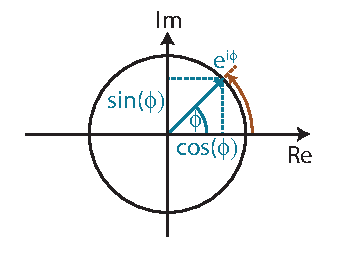
\includegraphics[width=0.4\textwidth]{Figures/complex_numbers.pdf}
        \caption{Komplexe Zahl $e^{i\phi}$ dargestellt als Vektor in der komplexen Zahlenebene. Wir können diese Zahl in Real- und Imaginärteil zerlegen, $e^{i\phi} = \cos{(\phi)} + i \sin{(\phi)}$. Wenn die Phase $\phi$ linear zeitabhängig ist, rotiert der Zahlenvektor gegen den Uhrzeigersinn.  }
        \label{fig:complexNumbers}
\end{figure}

Im Folgenden benötigen wir Exponentialfunktionen mit komplexen Argumenten, um Oszillationen darzustellen. Wir erinnern uns an die folgenden Reihenentwicklungen:
\begin{align}
&e^{\phi} = 1 + \phi + \frac{\phi^2}{2!} + \frac{\phi^3}{3!} + ... \nonumber\\
&\cos{\phi} = 1 - \frac{\phi^2}{2!} + \frac{\phi^4}{4!} - ...\nonumber\\
&\sin{\phi} = \phi - \frac{\phi^3}{3!} + \frac{\phi^5}{5!} - ...\,.
\label{eq:vl7a-1}
\end{align}
Hier nennen wir $\phi$ eine ``Phase''. Durch Einsetzen können wir überprüfen, dass ausserdem gilt
\begin{align}
&e^{i\phi} = \cos{\phi} +i\sin{\phi}\,.
\label{eq:vl7a-2}
\end{align}
Wenn die Phase linear von der Zeit abhängig ist, setzen wir $\phi = \omega t$ ein und erhalten eine Rotation in Gegenuhrzeigersinn in der komplexen Ebene:
\begin{align}
&e^{i\omega t} = \cos{\omega t} +i\sin{\omega t}\,.
\label{eq:vl7a-3}
\end{align}
Generell führen zeitabhängige reelle Argumente in der Exponentialfunktion entweder zu einem Wachstum oder einer Abnahme, je nach Vorzeichen. Imaginäre Argumente dagegen führen zu einer Oszillation. Die Form in \cref{eq:vl7a-3} ist sehr praktisch, um harmonische Oszillationen darzustellen, da man den Realteil der Funktion mit der Auslenkung $x(t)$ identifizieren kann und den Imaginärteil mit der entsprechenden zeitlichen Ableitung $\dot{x}/\omega$ (die Teilung durch $\omega$ ist nötig, um dieselbe Einheit wie für $x$ zu erhalten). Damit das Vorzeichen der Ableitung stimmt, benutzen wir für die Darstellung harmonischer Oszillatoren oft
\begin{align}
&e^{-i\omega t} = \cos{\omega t} -i\sin{\omega t}\,.
\label{eq:vl7a-4}
\end{align}
Das negative Vorzeichen entspricht einer Rotation in der komplexen Ebene im Uhrzeigersinn.

\subsection{Die Diskrete Fouriertransformation (DFT)}
\label{subsec:vl7}

Sei $x(t)$ eine Timetrace (d.h. gemessene Werte als Funktion der Zeit). 
Können wir die verschiedenen Frequenz-Komponenten dieses Signals einfach darstellen?  
Dafür ist folgendes Theorem wichtig: 
% und $R_{xx} (\tau)$ die zugehörige Auto-Kovarianz aus \cref{eq:AutokovarianzDeskret}, welche Information über die periodischen Signale in $x(t)$ wiedergibt. Gibt es eine Möglichkeit, die in $R_{xx} (\tau)$ enthaltenen Frequenzen einfach auszulesen?

\begin{center}
\begin{tcolorbox}[enhanced,width=6in,drop fuzzy shadow southwest,
    colframe=red!50!black,colback=red!05]
   Fouriers Theorem: Jede integrierbare Funktion kann als Summe von trigonometrischen Funktionen dargestellt werden.
\end{tcolorbox}
\end{center}


Diese Theorem führt zur \textbf{Fouriertransformation}. In dieser Vorlesung beschäftigen wir uns insbesondere mit der diskreten Fouriertransformation (DFT), da alle gemessen Signale sowohl in der Zeit als auch in der Auslenkung diskret sind (d.h., nur gewisse Werte annehmen). 
Mit der Exponentialschreibweise nimmt die DFT eines Signals $x(t)$ de folgende Form an: 

\begin{equation}
    x(t_k)= \sum_{n=-N/2}^{N/2} X(f_n) e^{i 2 \pi f_n t_k} 
\label{eq:vl7-1a}
\end{equation}

wobei $\Delta_f=1/t_\mr{tot}$ die kleinste Frequenzdifferenz ist, die in der Messzeit $t_\mr{tot}$ aufgelöst werden kann, und $f_n = n \Delta_f$ ist die $n$-te diskrete Frequenz, die wir als Funktion der diskreten Zeit $t_k = k\Delta_t$ betrachten. \\
Die komplexen Koeffizienten $X(f)$ geben an, wie gross die Amplitude der DFT an einer bestimmten Frequenz ist. Diese Koeffizienten können mit einer Rücktransformation bestimmt werden: 
\begin{equation}
    X(f_n)= \frac{1}{N}\sum_{k=0}^{N-1} x(t_k) e^{-i 2 \pi f_n t_k} 
\label{eq:vl7-1b}
\end{equation}
Wir können die $X(f_n)$ als Kovarianz zwischen dem Signal $x(t)$ und einem Testsignal $e^{-i 2 \pi f_n t_k}$ an der Frequenz $f_n$ vorstellen. $X(f_n)$ gibt also an, wie gut die beiden Signale übereinstimmen. Ob die Normierung $1/N$ in der Hin- oder in der Rücktransformation erfolgt, ist frei wählbar (es müssen aber andere Formeln entsprechend angepasst werden, siehe unten).
Abb. \ref{fig:fouriertransformation} zeigt ein Beispiel für eine Fouriertransformation.   \\

\begin{figure}[htbp]
    \centering
        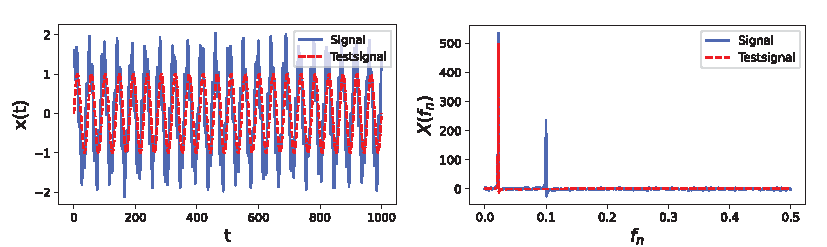
\includegraphics[width=\textwidth]{Figures/psd_fig1.pdf}
        \caption{Beispiel Fouriertransformation: Das gemessen Signal enthält zwei dominante Frequenzkomponenten, von denen eine mit dem Testsignal übereinstimmt. \textbf{Links:} Signal $x(t)$ and Testsignal $e^{i2\pi f_n t_k}$ \textbf{Rechts:} Fouriertransformation von $x(t_k)$ und vom Testsignal.}
        \label{fig:fouriertransformation}
\end{figure}
% Sei $F(x)$ eine integrierbare kontinuierliche Funktion. Dann ist $\tilde{F}(\xi)$ deren Fouriertransformierte (und umgekehrt). Es gilt:
% \begin{align}
% \tilde{F}(\xi)= \int_{-\infty}^{\infty} F(x) e^{-i 2 \pi \xi x}dx \nonumber\\
% {F}(x)= \frac{1}{2\pi}\int_{-\infty}^{\infty} \tilde{F}(\xi) e^{i 2 \pi \xi x}d\xi\,.
% \label{eq:vl7-1a}
% \end{align}
% Im Fall von diskreten Signalen definieren wir analog die diskrete Fouriertransformation (DFT) für die Funktion $F(x)$:
% \begin{align}
% \tilde{F}(\xi)= \sum_{n=0}^{N} F(x) e^{-i 2 \pi \xi x} \Delta x \nonumber\\
% {F}(x)= \frac{1}{2\pi}\sum_{n=0}^{N} \tilde{F}(\xi) e^{i 2 \pi \xi x}\Delta\xi\,,
% \label{eq:vl7-1b}
% \end{align}
% wobei $\Delta x$ (bzw. $\Delta \xi$) die Schrittgrösse in der jeweiligen Variable ist. 
Man beachte, dass die rein mathematische Definition der DFT für eine einheitenlose Zahlenfolge $x_n$ einfacher aussieht:
\begin{align}
X_k = \sum_{n=0}^{N-1} x_n e^{-i 2 \pi k n/N}\,.
\label{eq:vl7-1c}
\end{align}
Hier sind sowohl $x_n$ als auch die transformierte Zahlenfolge $X_k$ Zahlen ohne physikalische Bedeutung. Die Schrittgrösse, welche die Rolle einer diskreten Integrationsvariablen einnimmnt, reduziert sich hier auf $1$ und wird unsichtbar. Diese Formel kann also nicht direkt auf physikalische Signale mit Einheiten angewendet werden. In Python, MATLAB oder anderen Programmen, wo die Fouriertransformation mit Hilfe der ``fast Fourier transform'' FFT (einer effizienten Variante der DFT) berechnet wird, muss man daher das Resultat der FFT nachträglich mit der Schrittgrösse normieren. Generell ist immer Vorsicht geboten, wenn man einen Software-Algorithmus zum ersten Mal verwendet, da die Normierung nicht immer gleich implementiert ist. Im numpy-Paket von Python entspricht beispielsweise die funktion numpy.fft in unserer Notation nicht $X(f_n)$, sondern $NX(f_n)$. Man berechnet dann den spektralen Koeffizienten $X(f_n)$ einer Messreihe $x(t)$ mit dem folgenden Code: 
\begin{lstlisting}[language = Python]
FFTx = np.fft.fft(x)/N # fast Fourier transform von x(t) mit N Messwerten
Xn = FFTx[n] # Fourierkoeffizient mit Index n (fuer Details siehe Dokumentation)
\end{lstlisting}

Die Fouriertransformation kann entweder nur für positive (einseitig, single-sided) oder für positive und negative Frequenzen (zweiseitig, double-sided) definiert werden. In der zweiseitigen DFT eines Signals mit $N$ Punkten in der Zeit liegen im Frequenzraum ebenfalls $N$ Punkte vor, die zwischen den maximalen Frequenzen $\pm f_{max}$ (siehe unten) verteilt sind. Negative Frequenzen haben keine zusätzliche Bedeutung; die Fouriertransformation ist symmetrisch im Realteil (bzw. antisymmetrisch im Imaginärteil). Aus diesem Grund werden die negativen Frequenzanteile oft weggelassen und man erhält $N/2$ Punkte zwischen null und $f_{max}$.

\subsection{Eigenschaften der DFT}
\begin{itemize}
\item \textbf{Maximale Frequenz}: Die maximale Frequenz, die ohne Aliasing gesampelt werden kann, ist die sogenannte Nyquist-Frequenz:
        \begin{align}
        f_{max} = \frac{ 1 }{ 2 \Delta_t }\,.
        \label{eq:vl7-4}
        \end{align}
        Signale höherer Frequenz können mit derselben Samplingrate nicht richtig interpretiert werden und erzeugen im Spektrum Spitzen bei falschen Frequenzwerten.
        \begin{center}
        \begin{tcolorbox}[enhanced,width=6in,drop fuzzy shadow southwest,
            colframe=red!50!black,colback=red!05]
           Diese Limite für korrekt gemessene Frequenzen nennt man das Nyquist-Kriterium.
        \end{tcolorbox}
        \end{center}
        \item \textbf{Frequenzaufl\"osung}: Frequenzen können unterschieden werden, wenn über die gesamte Messzeit $t_\mr{tot}=N\Delta t$ mindestens eine volle Oszillation Unterschied entsteht, also $\Delta_t \leq 1/t_\mr{tot}$. Damit erhalten wir die Aufl\"osung:
        \begin{align}
        \delta f  = \frac{ 1 }{t_{tot}} = \frac{ 1 }{ N \Delta_t} = \frac{ 2 f_{max} }{ N }
        \label{eq:vl7-6}
        \end{align}
        mit $N$ Punkten von $-f_{max}$ bis $+f_{max}$. Die Frequenzwerte, an denen die DFT ausgwertet wird, entsprechen einer ganzen Zahl $n$ mal der Aufl\"osung:
        \begin{align}
        f_n = n \times \Delta_f\,.
        \label{eq:vl7-7}
        \end{align}
        \item Die PSD einer perfekten, unendlich lange gemessenen Sinuswelle hat einen einzelnen Peak bei der Wellenfrequenz und ist überall sonst gleich null. Perfektes weisses Rauschen hat über das gesamte Spektrum denselben Wert.
\end{itemize}

% Die Fouriertransformierte ist generell komplexwertig, wobei die Phase der komplexen Zahl $X(f_k)$ (bei einem bestimmten Wert von $\xi$) der Phase des Signals entspricht. Der reelle Teil von $\tilde{F}(\xi)$ gibt also den Cosinus-Anteil an, der imaginäre Teil den Sinus-Anteil. \\

% Angewendet auf unsere experimentelle Zahlenfolge $x(t)$, sieht das so aus: 
% \begin{equation}
%     x(t) = \sum_{n=-\infty}^{\infty} c_n e^{in2\pi\Delta_f t}~,
% \end{equation}
% wobei $\Delta_f=\frac{1}{t_{tot}}$ die kleinste Frequenz(differenz) ist, die in der Messzeit $t_{tot}$ aufgelöst werden kann. 
% Die komplexen Koeffizienten $c_n$ können mit einer Fouriertransformation bestimmt werden: 
% \begin{align}
%     c_n(f) & = \frac{1}{t_{tot}} \int_{t=0}^{t_{tot}} x(t) e^{-i2\pi f t} dt & \mathrm{Kontinuierliche~Fouriertransformation} \\
%     c_n(f) & =  \frac{1}{t_{tot}} \sum_{n=0}^N x(n\Delta_t) e^{-i2\pi f n \Delta_f} \Delta_t & \mathrm{Diskrete~Fouriertransformation} 
% \end{align}

\section{Die Spektrale Leistungsdichte}\label{sec:WienerKhinchin}

%\subsection{Die Spektrale Leistungsdichte -- Power Spectral Density (PSD)}
%\label{subsec:vl7-2}

In vielen Anwendungen sind wir nicht an der Phase oder dem Vorzeichen einer Fourierkomponente interessiert, sonder nur daran, wieviel Leistung in einem bestimmten Frequenzintervall enthalten ist. Beispielsweise kann es wichtig sein, wiviel Leistung eine Lichtquelle im sichtbaren Teil des elektromagnetischen Spektrums abstrahlt. In derartigen Fällen wird das normierte Quadrat der Fouriertransformation verwendet – die sogenannte Leistungsdichte oder power spectral density (PSD):
\begin{align}
S_{xx} (f) = \frac{\Delta_t}{N} \left| \sum_{k=0}^{N-1} x(t_k) e^{-i 2 \pi f_n t_k} \right|^2 = \Delta_t
N \left| X(f_n) \right|^2 \,,
\label{eq:vl7-3}
\end{align}
Mit Python lässt sich die gesamte PSD aller Frequenzen beispielsweise so berechnen:
\begin{lstlisting}[language = Python]
FFTx = np.fft.fft(x)/N # normierte FFT von x(t), d.h. Liste von Fourierkoeffizienten von x(t) mit N Messwerten
PSD = dt*N*np.abs(FFTx)**2
\end{lstlisting}


% \begin{figure}[htbp]
%     \centering
%     \begin{subfigure}[b]{0.49\textwidth}
%         \includegraphics[width=\textwidth]{Figures/psd-fig2.pdf}
%         \caption{Signal $x(t)$ mit gemessenen Punkten angenommen wir messen einmal pro s }
%         \label{fig:PSD_sub1}
%     \end{subfigure}
%     \hfill
%     \begin{subfigure}[b]{0.49\textwidth}
%         \includegraphics[width=\textwidth]{Figures/psd-fig3.pdf}
%         \caption{PSD der gemessenen Punkte (siehe .ipynb zu dieser Sektion)}
%         \label{fig:PSD_sub2}
%     \end{subfigure}
%     \caption{Beispiel PSD}
%     \label{fig:PSD}
% \end{figure}

\begin{figure}[htbp]
    \centering
        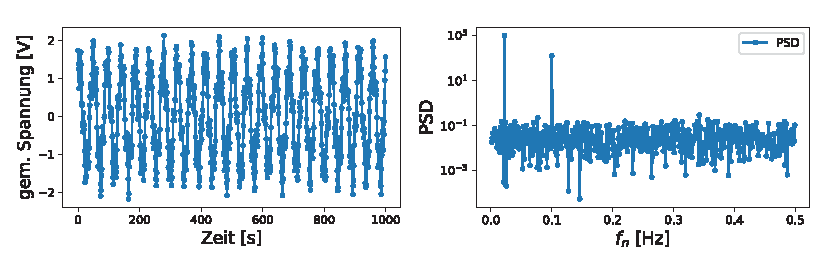
\includegraphics[width=\textwidth]{Figures/psd_fig2.pdf}
        \caption{Beispiel PSD. \textbf{Links:} Signal $x(t)$ mit gemessenen Punkten angenommen wir messen einmal pro s  \textbf{Rechts:} PSD der gemessenen Punkte (siehe .ipynb zu dieser Sektion)}
        \label{fig:PSD}
\end{figure}

Die PSD kann auch anders berechnet werden: Wenn wir die Fouriertransformation der Auto-Kovarianz $R_{xx}(t)$ aus Gl. (\ref{eq:AutokovarianzDeskret}) bilden, erhalten wir die spektrale Leistungsdichte (power spectral density, \gls{gl:PSD}) \gls{gl:S_xx}:

\begin{align}
S_{xx} (f) = \sum_{n=0}^{N} R_{xx} (\tau_n) e^{-i 2 \pi f \tau_n}\Delta \tau
\label{eq:vl7-1}
\end{align}
mit der entsprechenden Rücktransformation
\begin{align}
R_{xx} (\tau) = \frac{1}{2 \pi} \sum_{n=0}^{N} S_{xx} (f_n) e^{i 2 \pi f_n \tau}\Delta f\,.
\label{eq:vl7-2}
\end{align}

\begin{center}
\begin{tcolorbox}[enhanced,width=6in,drop fuzzy shadow southwest,
    colframe=red!50!black,colback=red!05]
   Dieser Zusammenhang zwischen der Auto-Kovarianz und der spektralen Leistungsdichte ist bekannt als das Wiener-Khinchin Theorem.
\end{tcolorbox}
\end{center}

 

Abb. \ref{fig:PSD} zeigt, wie wir das Signal $x(t)$ aus dem vorherigen Kapitel mit einem Analog-Digital-Konverter messen und dann die PSD dieser Messung berechnen. \\ 

Die Normierung mit $\Delta_t$ in Gl. (\ref{eq:vl7-3}), bzw. $\Delta_\tau$ in Gl. (\ref{eq:vl7-1}) macht aus einem Power Spectrum (mit derselben Einheit wie $x^2$) eine PSD mit der Einheit $x^2/$Hz (zum Beispiel $m^2/$Hz, $V^2/$Hz, ...). 
%\textit{Beispiel: Die PSD einer perfekten Sinuswelle hat einen Peak bei der Signalfrequenz und ist sonst \"uberall Null.}

%\begin{center}
%\textcolor{red}{Wir betrachten die Leistung (Power), also das Quadrat der diskreten Fourier-Transformation (\gls{gl:DFT}), da die Power unabh\"angig vom Vorzeichen und damit einfacher auszulesen ist.}
%\end{center}

%Weiterhin betrachten wir die spektrale Dichte anstatt dem Powerspektrum (\gls{gl:PS}, mit derselben Einheit wie $x^2$), da der PSD-Wert ($S_{xx}$) unabhängig von der Messzeit und oft relevanter als das Powerspektrum ist. Die Normierung mit $\delta t$ macht aus einem Powerspektrum eine PSD mit der Einheit $V^2$/Hz, $m^2$/Hz, $I^2$/Hz. Der gemessene Wert der PSD hängt nicht von der Frequenzauflösung ab (im Gegensatz zur PS). Eine lange und eine kurze Messung sollen dasselbe Resultat produzieren!


\subsection{Eigenschaften der spektralen Leistungsdichte (PSD)}
\label{subsec:vl7-3}

%Ist der Zeitintervall zwischen Messpunkten $\delta t \ll 1/f_{signal}$, so wird die Signalfrequenz korrekt gemessen. Ist aber der Zeitintervall zwischen Messpunkten $\delta t > 1/f_{signal}$, kann die Signalfrequenz nicht korrekt gemessen werden und diesem Fall kommt es zum ``Aliasing''.
\begin{itemize}
    \setlength\itemsep{0em}
        \item Die PSD bildet das Spektrum der Leistung, welche im Gegensatz zur Amplitude der Welle nicht von der Wellenphase abhängt. Die PSD ist also überall positiv.
        \item Die Normierung der PSD ist so gewählt, dass ihre numerische Integration über alle Frequenzen der Varianz $\sigma_x^2$ entspricht (siehe ``Parseval-Theorem'' in Sektion~\ref{subsec:vl7-4}). Deshalb muss die PSD Einheiten von $x^2/Hz$ haben. Im Gegensatz zum Leistungsspektrum, welches auch oft verwendet wird, ist der Wert der PSD an einer bestimmten Frequenz unabhängig von der Messzeit (abgesehen von statistischen Fehlern).
        \item Die PSD ist generell für positive und negative Werte von $f$ bestimmt und symmetrisch um $f=0$. Oft wird nur der positive Teil der PSD gezeigt. Dann muss die PSD mit einem Faktor 2 multipliziert werden, um die Normierung zu erhalten. Es wird deshalb immer angegeben, ob man die ``single-sided'' oder ``double-sided PSD'' benutzt.
\end{itemize}

\section{Rauschen und Parsevals Theorem}\label{sec:Parseval}
\begin{center}
\begin{tcolorbox}[enhanced,width=6in,center upper,
    fontupper=\large,drop fuzzy shadow southwest,
    colframe=blue!50!black,colback=blue!10]
    {Zu Rauschen und Parseval-Theorem ist ein Jupyter-Notebook verfügbar. Siehe \gitresource{Parseval theorem and filtering.ipynb} }
\end{tcolorbox}
\end{center}
\subsection{Parseval-Theorem}
\label{subsec:vl7-4}

Die wichtige Normierungseigenschaft der PSD, welche einen Zusammenhang zwischen der Varianz einer Variable $x(t)$ und dessen PSD herstellt, ist bekannt als das Parseval-Theorem. F\"ur 
den kontinuierlichen, doppelseitig definierten Fall lautet das Parseval-Theorem:
\begin{align}
\sigma_x^2 = \int_{- \infty}^\infty S_{xx} (f) df\,,
\label{eq:vl7-8}
\end{align}
F\"ur den diskreten, doppelseitig definierten Fall entspricht dies:
\begin{align}
\sigma_x^2 = \Delta_f \sum_{f = -f_{max}}^{f_{max}} S_{xx} (f)\,.
\label{eq:vl7-9}
\end{align}
Wenn einseitig definierte PSDs verwendet werden, muss ihr Wert mit einem Faktor 2 multipliziert werden, damit das Integral (bzw. die Summe) von null bis $f_{max}$ immer noch der Varianz entspricht.

Die PSDs unkorrelierter Variablen sind additiv, also gilt für ein Signal $x(t) = a(t) + b(t)$
\begin{equation}
        S_{xx}(f_n) = S_{aa}(f_n) + s_{bb}(f_n) \,.\label{eq:additive_PSDs}
\end{equation}
Aus dem Parseval-Thereom und Gl. (\ref{eq:additive_PSDs}) folgt dann die bereits bekannte Tatsache, dass auch die Varianzen unkorrelierter Variablen additiv sind, also 
\begin{equation}
    \sigma_x^2 = \sigma_a^2 + \sigma_b^2\,.
\end{equation}
Diese Eigenschaft können wir uns zunutze machen, um zum Beispiel ein bekanntes Detektorrauschen von einem unbekannten Signal abzuziehen, wie in der Vorlesung gezeigt. 

\subsection{Rauschen in der PSD}
\label{subsec:vl10}

% \begin{figure}[htbp]
%     \centering
%     \begin{subfigure}[b]{0.49\textwidth}
%         \includegraphics[width=\textwidth]{Figures/parseval_fig3.pdf}
%         \caption{Signal $x(t)$ mit unbekannten Frequenzkomponenten in blau und gefiltertes Signal in rot}
%         \label{fig:parseval_sub1}
%     \end{subfigure}
%     \hfill
%     \begin{subfigure}[b]{0.49\textwidth}
%         \includegraphics[width=\textwidth]{Figures/parseval_fig4.pdf}
%         \caption{PSD von $x(t)$ in blau und vom gefilterten Signal in rot. Die Frequenzkomponente bei 15.75\,Hz ist besonders ausgeprägt und der Tiefpassfilter macht diese Frequenz besser sichtbar.  }
%         \label{fig:parseval_sub2}
%     \end{subfigure}
%     \caption{Beispiel Rauschen und Tiefpassfilter in der PSD}
%     \label{fig:parseval}
% \end{figure}


\begin{figure}[htbp]
    \centering
        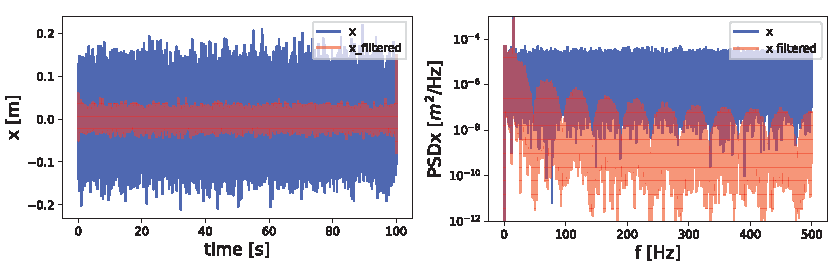
\includegraphics[width=\textwidth]{Figures/psd_fig3.pdf}
        \caption{Beispiel Rauschen und Tiefpassfilter in der PSD. \textbf{Links:} Signal $x(t)$ mit unbekannten Frequenzkomponenten in blau und gefiltertes Signal in rot/ \textbf{Rechts:} PSD von $x(t)$ in blau und vom gefilterten Signal in rot. Die Frequenzkomponente bei 15.75\,Hz ist besonders ausgeprägt und der Tiefpassfilter macht diese Frequenz besser sichtbar.}
        \label{fig:parseval}
\end{figure}

In Abb. \ref{fig:parseval} ist eine Messdatenreihe und ihre PSD zu sehen. Eine Frequenzkomponente bei 15.75\,Hz sticht im Spektrum heraus. Wir können einen \textit{Tiefpassfilter} anwenden, um das Rauschen bei allen anderen Frequenzen zu dämpfen und so das Signal auch im Zeitraum besser sichbar zu machen. 

Wir implementieren einen einfachen digitalen Tiefpassfilter, indem wir jeden Punkt in $x(t)$ mit seinen 10 Nachbarn zu jeder Seite mitteln. Wie erwartet finedne wir, dass die PSD bei höheren Frequenzen deutlich reduziert wurde.\\ 

Nach Gl. (\ref{eq:vl7-9}) wurde durch das Filtern auch die Varianz des Signals verringert, was wir in Abb. \ref{fig:parseval} (links) anhand der Breite des roten gegenüber des blauen Signals qualitativ abschätzen können. \\

%Wenn wir durch das Mitteln verschiedener Frequenzkomponenten interessante Signale verwaschen, können wir stattdessen die Messung auch N Male wiederholen und jeden Punkt als Funktion der Zeit mitteln. 
%In beiden Fällen bilden wir einen Mittelwert und erhalten dementsprechend kleinere Fehler. 
In der gemittelten Messung entspricht jeder Punkt dem Mittelwerts aus mehreren ursprünglichen Messwerten. Dadurch werden die statistischen Fehler an jedem Punkt zu einem Fehler des Mittelwerts, und die Standardabweichung reduziert sich um $1/\sqrt{N}$. Die bedeutet auch, dass benachbarte Punkte (innerhalb der Filterzeit) miteinander korreliert werden, also nicht mehr unabhängige Information enthalten. Dieser Verlust an (hochfrequenten) Informationen ist genau der Effekt, den wir durch das Filtern erzielen wollen. Eine Reduktion des Rauschens geht also automatisch einher mit Informationsverlust.

% \textbf{Beispiel: }
% Sei $x(t)$ eine Timetrace (gemessene Werte als Funktion der Zeit) und $S_{xx}(f)$ die zugehörige PSD definiert zwischen $f=0$ und $f_{max} = 500$\,Hz (``einseitig'', vgl. \cref{subsec:vl7-2}). Falls die PSD ungefähr weiß (``flach'') ist, können wir die Varianz gemäß dem Parseval-Theorem sehr einfach berechnen (vgl. \cref{subsec:vl7-3} und \cref{subsec:vl7-4}):
% \begin{align}
%     \begin{split}
%         \sigma_x^2 &= \Delta_f \sum_{f = 0}^{f_{max}} S_{xx}(f)\\
%         &= \Bar{S}_{xx} f_{max}~,
%     \label{eq:vl10-1}
%     \end{split}
% \end{align}
% Wobei $\Bar{S}_{xx}$ der durchschnittlichen PSD entspricht, siehe Abbildung \textcolor{blue}{take lecture picture}. 
% Daraus sehen wir direkt, dass eine höhere Nyquist-Frequenz $f_{max}$ zu mehr Rauschen führt. Es kann daher von Vorteil sein, eine langsamere Messrate (Samplingrate) zu verwenden, um eine genauere Messung zu erhalten.
    
% \begin{center}
% \textbf{In vielen Situationen gilt die Faustregel: Eine längere und/oder langsamere Messung ist genauer als eine kurze und schnelle Messung.}
% \end{center}


\subsection{Filterarten}
\label{subsec:vl10-2}

Wie in der letzten Sektion gezeigt, kann man Filter einsetzen, um verschiedene Frequenzanteile eines Signals herauszufiltern. Im Wesentlichen unterscheidet man drei Filterarten:
\begin{itemize}
\setlength\itemsep{0em}
    \item Tiefpass (low-pass): Hohe Frequenzanteile werden abgeschw\"acht, niedrige Frequenzanteile werden transmittiert.
    \item Bandpass (band-pass): Frequenzanteile ausserhalb eines bestimmten Frequenzbereiches werden abgeschw\"acht, der Band-Frequenzbereich wird transmittiert.
    \item Hochpass (high-pass): Niedrige Frequenzanteile werden abgeschw\"acht, hohe Frequenzanteile werden transmittiert.
\end{itemize}

\begin{figure}[tbp]
    \centering
        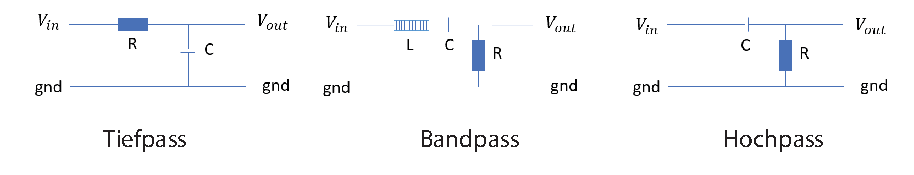
\includegraphics[width=\textwidth]{Figures/filter.pdf}
        \caption{Analoge Implementierung von verschiedenen Filtern. \textbf{Links:} Tiefpass aus paralleler Kapazität \textbf{Mitte:} Bandpass aus serieller Induktivität und Kapazität \textbf{Rechts:} Hochpass aus serieller Kapazität}
        \label{fig:analogueFilters}
\end{figure}

%\textit{Beispiel: Es sei ein Signal mit einer Grundfrequenz von 100\,Hz geben das \"Uberlagerungen h\"oherer und niedriger Frequenzen aufweist (und daher von der Idealform eines Sinus abweicht). Ein Low-pass-Filter mit der Grenzfrequenz $f_{3\,\text{dB}} =$ 150\,Hz schw\"acht alle Frequenzen \"uber 150\,Hz ab, w\"ahrend Frequenzen unterhalb von 150\,Hz mit nahezu maximaler Amplitude durchgelassen werden. Dabei betr\"agt die Abschw\"achung bei 150 Hz 3\,dB. Dadurch wird das urspr\"ungliche Signal entsprechend ``gegl\"attet''. Hingegen transmittiert ein Band-pass-Filter mit $f_{band} =$ 100\,Hz beispielsweise nur einen Frequenzbereich von 50 - 150\,Hz.}\\[0.3 cm]
%Die Ansprechzeit, sprich Wartezeit von Filtern ist direkt proportional zur Frequenz $f$:
% \begin{align}
    %\begin{split}
       % \text{Low-/High-pass: } \tau_{av} &\approx \frac{1}{2 \pi f_{3\,\text{dB}}}\\
        %\text{Band-pass: } \tau_{av} &\approx \frac{1}{\pi f_{3\,\text{dB}}}
        %\label{eq:vl10-3}
    %\end{split}
%\end{align}

Derartige Filter lassen sich digital als Algorithmen oder analog durch elektronische Bauteile implementieren. Die einfachsten analogen, elektronischen Varianten sind, siehe Abb. \ref{fig:analogueFilters}:
\begin{itemize}
\setlength\itemsep{0em}
    \item Low-pass: Widerstand und Kondensator
    \item Band-pass: Spule, Kondensator und Widerstand (ein RLC Resonator)
    \item High-pass: Kondensator und Widerstand
\end{itemize}

Wir betrachten Als Beispiel den typischen RC-Tiefpassfilter, der aus einem Widerstand $R$ in der Signalleitung und einer Kapazität $C$ zur Erdung besteht (siehe Zeichnung in Vorlesungs-Slides). Die Impedanzen (``komplexen Widerst\"ande'') der Elemente $R$ und $C$ sind in Abh\"angigkeit der Signalfrequenz $\omega$ gegeben als:
\begin{align}
    \begin{split}
        Z_R &= R\\
        Z_C &= \frac{1}{i \omega C}\,.
        \label{eq:vl10-4}
    \end{split}
\end{align}

Das Verh\"altnis $T_{filter}$ der Ein- und Ausgangsspannungen $V_{in} = I_{in} (Z_R + Z_C)$ bzw. $V_{out} = I_{in} Z_C$, l\"asst sich wie folgt bestimmen:
\begin{align}
    \begin{split}
        T_{filter} &= \frac{|V_{out}|^2}{|V_{in}|^2}\\
        &= \frac{|Z_C|^2}{|R + Z_C|^2}\\
        &= \frac{1/(\omega C)^2}{R^2 + 1/(\omega C)^2}\\
        &= \frac{1}{1 + (\omega R C)^2}\\
        &= \frac{1}{1 + \omega^2 / \omega_{3\,\text{dB}}^2}\,.
        \label{eq:vl10-5}
    \end{split}
\end{align}

Hierbei ist $\omega_{3\,\text{dB}} = 1/RC$ die Frequenz, bei der $|V_{out}|^2$ den halben Wert von $|V_{in}|^2$ erreicht.\\[0.3 cm]

%Die digitale Implementierung hat folgende Form::
%\begin{itemize}
%\setlength\itemsep{0em}
%    \item Low-pass: $y(n) = x(n) + x(n-1)$ (Fehler des Mittelwerts)
%    \item Band-pass: $y(n) = \underbrace{L_1(n)}_{\text{Low-pass @ } f_1} + %\underbrace{H_2(n)}_{\text{High-pass @ } f_2}$
%    \item High-pass: $y(n) = \underbrace{A(n)}_\text{All-pass} - \underbrace{L(n)}_\text{Low-pass}$
%\end{itemize}


%Es gilt: Reduziere die Unsicherheit (des gemessenen Wertes $S_{xx}$) für jeden Frequenzpunkt durch wiederholte Messungen. Wir erhalten einen ``Fehler des Mittelwertes'' für jeden Wert von $S_{xx} (f)$.

\newpage

\begin{tcolorbox}[enhanced,width=6in,
    fontupper=\small,drop fuzzy shadow southwest,
    colframe=black!50!black,colback=black!5]
\textbf{Verständnisfragen:} \\
\begin{enumerate}
\item[1] Was besagt Fouriers Theorem?
\item[2] Wann würden wir typischerweise die kontinuierliche/diskrete Fouriertransformation benutzen?
\item[3] Was ist die maximale Frequenz, die ohne Aliasing gesampelt werden kann?
\item[4] Was besagt das Parseval-Theorem und warum ist es wichtig? 
\item[5] Wie berechnet man die Standardabweichung $\sigma_x$ eines rauschbehafteten Signals x(t)?
\item[6] Welche Frequenzanteile werden durchgelassen wenn erst ein Hochpass, und dann ein Tiefpassfilter angewendet wird? 
\end{enumerate}
\end{tcolorbox}

\begin{tcolorbox}[enhanced,width=6in,
    fontupper=\small,drop fuzzy shadow southwest,
    colframe=black!50!black,colback=black!5]
\textbf{Antworten:} \\
\begin{enumerate}
\item[1] Fouriers Theorem besagt das jede integrierbare Funtion als Summe von trigonometrischen Funktionen dargestellt werden kann. 
\item[2] Beim Herleiten von analytischen Zusammenhängen verwendet man oft die kontinuierliche Fouriertransformation, und beim analysieren von experimentellen Daten verwendet man im Regelfall die diskrete Fouriertransformation, da eine gespeicherte Messunge aus diskreten Datenpunkten besteht.  
\item[3] Die Nyquist-Frequenz, $f_{max} = 1/2\delta t$
\item[4] Das Parseval-Theorem besagt, dass das Integral über die PSD der Varianz entspricht. Dies ist wichtig zur Normierung der PSD. 
\item[5] Über das Parseval-Theorem lässt sich die Varianz $\sigma_x^2$ aus der PSD berechnen. Die Standardabweichung ist dann $\sqrt{\sigma_x^2}$. 
\item[6] Wenn sich die Frequenzbereiche des Hoch- und Tiefpasses überschneiden, werden diejenigen Frequenzen durchgelassen, die in dem Überschneidungsbereich liegen, ähnlich wie bei einem Bandpass. Wenn sich die Frequenzen der beiden Filter nicht überschneiden, wird kein Signal durchgelassen. 
\end{enumerate}
\end{tcolorbox}